%\documentclass[11pt,letterpaper]{article}
\documentclass[oneside,11pt]{amsart}

%\usepackage{a4wide}
%\usepackage{epsfig}
%\usepackage{psfig}
\usepackage{graphicx}
\usepackage{natbib,latexsym,url,enumitem,pdfpages}
\usepackage{color}
\usepackage{wrapfig}
\usepackage{caption}

\captionsetup{
    justification=justified,
    margin=0pt,
    font=small}

% Some fancy commenting
\definecolor{todo}{RGB}{200,0,0}
\newcommand{\comment}[2][todo]{{\color{#1}[[{\bf #2}]]}}

% Challenge counter
\newcounter{chalno}
\newcommand{\chal}[1]{\refstepcounter{chalno}\label{#1}}

% User commands
\makeatletter
\let\jnl@style=\rm
\def\ref@jnl#1{{\jnl@style#1}}

\def\ref@jnl#1{{\jnl@style#1}}% 
\newcommand\aj{\ref@jnl{AJ}}%        % Astronomical Journal 
\newcommand\araa{\ref@jnl{ARA\&A}}%  % Annual Review of Astron and Astrophys 
\newcommand\apj{\ref@jnl{ApJ}}%    % Astrophysical Journal ++
\newcommand\apjl{\ref@jnl{ApJL}}     % Astrophysical Journal, Letters 
\newcommand\apjs{\ref@jnl{ApJS}}%    % Astrophysical Journal, Supplement 
\newcommand\ao{\ref@jnl{ApOpt}}%   % Applied Optics ++
\newcommand\apss{\ref@jnl{Ap\&SS}}%  % Astrophysics and Space Science 
\newcommand\aap{\ref@jnl{A\&A}}%     % Astronomy and Astrophysics 
\newcommand\aapr{\ref@jnl{A\&A~Rv}}%  % Astronomy and Astrophysics Reviews 
\newcommand\aaps{\ref@jnl{A\&AS}}%    % Astronomy and Astrophysics, Supplement 
\newcommand\azh{\ref@jnl{AZh}}%       % Astronomicheskii Zhurnal 
\newcommand\baas{\ref@jnl{BAAS}}%     % Bulletin of the AAS 
\newcommand\icarus{\ref@jnl{Icarus}}% % Icarus
\newcommand\jrasc{\ref@jnl{JRASC}}%   % Journal of the RAS of Canada 
\newcommand\memras{\ref@jnl{MmRAS}}%  % Memoirs of the RAS 
\newcommand\mnras{\ref@jnl{MNRAS}}%   % Monthly Notices of the RAS 
\newcommand\pra{\ref@jnl{PhRvA}}% % Physical Review A: General Physics ++
\newcommand\prb{\ref@jnl{PhRvB}}% % Physical Review B: Solid State ++
\newcommand\prc{\ref@jnl{PhRvC}}% % Physical Review C ++
\newcommand\prd{\ref@jnl{PhRvD}}% % Physical Review D ++
\newcommand\pre{\ref@jnl{PhRvE}}% % Physical Review E ++
\newcommand\prl{\ref@jnl{PhRvL}}% % Physical Review Letters 
\newcommand\pasp{\ref@jnl{PASP}}%     % Publications of the ASP 
\newcommand\pasj{\ref@jnl{PASJ}}%     % Publications of the ASJ 
\newcommand\qjras{\ref@jnl{QJRAS}}%   % Quarterly Journal of the RAS 
\newcommand\skytel{\ref@jnl{S\&T}}%   % Sky and Telescope 
\newcommand\solphys{\ref@jnl{SoPh}}% % Solar Physics 
\newcommand\sovast{\ref@jnl{Soviet~Ast.}}% % Soviet Astronomy 
\newcommand\ssr{\ref@jnl{SSRv}}% % Space Science Reviews 
\newcommand\zap{\ref@jnl{ZA}}%       % Zeitschrift fuer Astrophysik 
\newcommand\nat{\ref@jnl{Nature}}%  % Nature 
\newcommand\iaucirc{\ref@jnl{IAUC}}% % IAU Cirulars 
\newcommand\aplett{\ref@jnl{Astrophys.~Lett.}}%  % Astrophysics Letters 
\newcommand\apspr{\ref@jnl{Astrophys.~Space~Phys.~Res.}}% % Astrophysics Space Physics Research 
\newcommand\bain{\ref@jnl{BAN}}% % Bulletin Astronomical Institute of the Netherlands 
\newcommand\fcp{\ref@jnl{FCPh}}%   % Fundamental Cosmic Physics 
\newcommand\gca{\ref@jnl{GeoCoA}}% % Geochimica Cosmochimica Acta 
\newcommand\grl{\ref@jnl{Geophys.~Res.~Lett.}}%  % Geophysics Research Letters 
\newcommand\jcp{\ref@jnl{JChPh}}%     % Journal of Chemical Physics 
\newcommand\jgr{\ref@jnl{J.~Geophys.~Res.}}%     % Journal of Geophysics Research 
\newcommand\jqsrt{\ref@jnl{JQSRT}}%   % Journal of Quantitiative Spectroscopy and Radiative Trasfer 
\newcommand\memsai{\ref@jnl{MmSAI}}% % Mem. Societa Astronomica Italiana 
\newcommand\nphysa{\ref@jnl{NuPhA}}%     % Nuclear Physics A 
\newcommand\physrep{\ref@jnl{PhR}}%       % Physics Reports 
\newcommand\physscr{\ref@jnl{PhyS}}%        % Physica Scripta 
\newcommand\planss{\ref@jnl{Planet.~Space~Sci.}}%  % Planetary Space Science 
\newcommand\procspie{\ref@jnl{Proc.~SPIE}}%      % Proceedings of the SPIE 

\newcommand\actaa{\ref@jnl{AcA}}%  % Acta Astronomica
\newcommand\caa{\ref@jnl{ChA\&A}}%  % Chinese Astronomy and Astrophysics
\newcommand\cjaa{\ref@jnl{ChJA\&A}}%  % Chinese Journal of Astronomy and Astrophysics
\newcommand\jcap{\ref@jnl{JCAP}}%  % Journal of Cosmology and Astroparticle Physics
\newcommand\na{\ref@jnl{NewA}}%  % New Astronomy
\newcommand\nar{\ref@jnl{NewAR}}%  % New Astronomy Review
\newcommand\pasa{\ref@jnl{PASA}}%  % Publications of the Astron. Soc. of Australia
\newcommand\rmxaa{\ref@jnl{RMxAA}}%  % Revista Mexicana de Astronomia y Astrofisica

%% added feb 9, 2016
\newcommand\maps{\ref@jnl{M\&PS}}% Meteoritics and Planetary Science
\newcommand\aas{\ref@jnl{AAS Meeting Abstracts}}% American Astronomical Society Meeting Abstracts
\newcommand\dps{\ref@jnl{AAS/DPS Meeting Abstracts}}% American Astronomical Society/Division for Planetary Sciences Meeting Abstracts



\let\astap=\aap 
\let\apjlett=\apjl 
\let\apjsupp=\apjs 
\let\applopt=\ao 



\DeclareRobustCommand{\gtrsim}{%
\mathrel{\hskip-.5em\begin{array}{c}>\\[-8pt]\sim\end{array}\hskip-.5em}}
\DeclareRobustCommand{\lesssim}{%
\mathrel{\hskip-.5em\begin{array}{c}<\\[-8pt]\sim\end{array}\hskip-.5em}}

\pretolerance=10000
\textwidth=6.4in
\textheight=8.95in
\voffset = 0.in
%\voffset = -0.3in  % For my printer
\topmargin=0.0in
\headheight=0.00in
\hoffset = 0.0in
%\hoffset = 0.33in  %  For my printer
\headsep=0.00in
\oddsidemargin=0in
\evensidemargin=0in
\parindent=2em
\parskip=0.2ex
 
\renewcommand{\baselinestretch}{1.03}

\special{papersize=8.5in,11in}

\newcommand{\markus}{\textcolor{green}}

\setlength{\parskip}{0.6 ex plus 0.4ex minus 0.2ex} \flushbottom
\pagestyle{plain} 

\begin{document}
% \thispagestyle{empty}

\pagenumbering{arabic}

\vspace*{-1.5cm}

\centerline{\textsf {\Large The FOBOS Spectroscopic Facility for Keck: Project Description}}


% \centerline{\textsf {\large Project Summary}}

% \bigskip
% \noindent {\bf Overview:} In this \emph{Design}
% submission, we propose to dramatically enhance the power of upcoming
% panoramic deep-imaging from the Large Synoptic Survey Telescope (LSST),
% Euclid and the Wide-Field Infrared Survey Telescope (WFIRST) in order to
% address key questions in the areas of dark energy, the galaxy ecosystem
% at $z\sim2$, and the assembly history of the Milky Way and Local Group
% Galaxies.  We will design the astrostatistics, instrumentation, and
% software solutions required over the next decade to provide optimized
% spectroscopic training sets that can unlock \emph{physical
% information} (e.g., redshifts, galaxy star formation histories, stellar
% metallicities) from deep photometry alone.  Applying machine learning to
% a set of ambitious Data Science Challenges using simulated data, we will define
% requirements on future spectroscopic training sets.  These requirements
% will guide the preliminary design of FOBOS, a powerful new spectrograph
% to deploy in 2026 on the 10 m Keck II Telescope.  FOBOS will provide
% publicly-available deep, high-multiplex spectroscopy with high target
% sampling and flexibility uniquely matched to the ``Big Data'' training
% problem.

% \bigskip
% \noindent {\bf Intellectual Merit:} High-multiplex and deep
% spectroscopic followup of LSST and other panoramic deep-imaging surveys
% is a widely recognized necessity.  Reports in 2015 and 2016 by the
% National Research Council and National Optical Astronomical Observatory
% specifically recommend that the NSF support construction of required
% spectroscopic facilities because none currently exist or are planned at
% U.S.\ observatories.  FOBOS satisfies these spectroscopic needs at
% relatively low cost by utilizing the existing 10 m Keck II Telescope, a
% highly-successful U.S.-led large telescope.  Even with the powerful capabilities of FOBOS deployed, the astronomical
% community recognizes the need for cutting-edge data science techniques to ``train''
% vast photometric surveys with what will necessarily be more limited
% spectroscopy.  Success in the training methodologies we propose here
% will make photometric redshifts more precise, improving the LSST dark
% energy figure-of-merit by 40\%.  They will enable a comprehensive
% understanding of galaxies and their gaseous environments at $z\sim2$,
% and they will reveal fossilized structures in the Milky Way, M31, and
% other Local Group galaxies through chemical signatures inferred for
% millions of stars.

% \bigskip
% \noindent {\bf Broader Impacts:} We will build on the success of several ongoing programs at UC Santa Cruz (UCSC) that
% connect high school and college students, especially those from underrepresented minorities, to active research groups.
% Studies show that such connections increase STEM retention.  The flagship program is Akamai, run by UCSC's Institute
% for Scientist and Engineer Educators (ISEE), which advances college students from Hawai'i into the STEM workforce.  Our
% proposal supports two Akamai interns to work at UCSC on instrument simulation and design as well as machine learning
% for spectroscopic analysis.  We will also engage a cohort of graduate students in ISEE's Professional Development
% Program which builds teaching skills as students develop an inquiry-based activity. The graduate students will then
% conduct this activity, centered on FOBOS instrument development, with 25 largely underrepresented community college
% students from UCSC's Lamat program.  Finally, we will take advantage of a successful hands-on research course and a
% long-running summer internship program to introduce data simulation and machine-learning techniques to 1st-year
% undergraduate and senior high school students.

% \clearpage


\setcounter{page}{1}

\centerline{{\it MSIP proposal category: ``Development Investments''}}

\section{Scientific Justification} 

\subsection{Introduction}
Led by NSF's LSST\footnote{
%
LSST: Large Synoptic Survey Telescope.  LSST will be begin science operations in 2023.}
%
and NASA-supported missions like Euclid\footnote{
%
Euclid is led by the European Space Agency with significant NASA involvement and will launch
in 2021. Its primary mission is a 15,000 deg$^2$ imaging survey in optical and near-IR wavebands.} 
%
and WFIRST\footnote{
%
WFIRST: The Wide Field Infrared Survey Telescope, expected to launch in the mid 2020's.},
%
astronomy is entering a new era of unprecedented deep-imaging campaigns that will survey huge volumes of the
Universe.  From the emergence of the earliest galaxies from a ``primordial soup'' of gas and dust, to the peak of
cosmic star formation and the current era of accelerated expansion, these surveys will provide unprecedented statistics
at key epochs of cosmic history.

% Meanwhile, the rate of cosmic expansion was beginning to accelerate,
% as the Universe became increasingly dominated by ``Dark Energy,''
% whose origin remains the single greatest mystery in astronomy and
% cosmology today.

% Since Edwin Hubble's observations over 100 years ago,

Even so, gaining physical insight from panoramic imaging surveys will require intensive spectroscopic follow-up.  The
power of combining photometry and dedicated spectroscopy is widely appreciated and perhaps best illustrated by the
success of the Sloan Digital Sky Survey (SDSS) which used this combination to record the properties of over 1 million
galaxies, mapping the present-day universe and making SDSS one of the most highly cited surveys in the history of
astronomy.

% Because a quality spectrum requires far more observing time per source
% than an image, SDSS pioneered ``high multiplex'' spectrographs,
% capable of \emph{simultaneous} spectroscopy of hundreds of objects.

LSST's all-sky images, for example, will be 1,000 times deeper and detect far more
distant galaxies than SDSS, but \textbf{no current U.S.~facility is
capable of obtaining spectroscopic follow-up of LSST galaxies} at a level
required to capitalize on the \$1B the U.S.\ has invested in that
project.  In fact, an SDSS-like spectroscopic study of 1 million
galaxies at LSST depth would require 300 years of observing on the
largest telescopes with current instrumentation!  

This proposal addresses this challenge through the design of an ambitious spectroscopy facility on one of the world's largest telescopes.  Timed to deploy on WMKO's\footnote{WMKO: W.~M.\ Keck Observatory operates the two twin 10m Keck Telescopes.} Keck II Telescope in 2028, just as various panoramic deep imaging surveys hit their stride, FOBOS's\footnote{FOBOS: Fiber-Optic Broadband Optical Spectrograph} 1800-fiber multiplex, deep sensitivity, high sampling density, and wide wavelength coverage is optimized for the \emph{deep-drilling} spectroscopic training sets required to extract maximum information from wide-field photometry.  Its flexible target allocation system and multiplexed IFU mode provide unique capabilities for realizing major progress on fundamental goals in Cosmology, Galaxy Formation, and Local Group Archaeology, and Time Domain Astronomy in the coming decade.

Based on science requirements derived from reference-mission key programs, we present a comprehensive plan for optimizing and completing the design of the FOBOS instrumentation, calibration and support systems, operational and planning software, and data management systems.  We propose community engagement activities to coordinate involvement of U.S.~astronomers including those outside the Keck Community in developing and leading FOBOS public survey programs whose data products will benefit wide swaths of the astronomical community.  In partnership with NOAO (this name might change), we will develop additional ``open-access'' models to offer $\sim$100,000 fiber-hours per year in support of individual, PI-led programs to be integrated into the FOBOS observing suite.  Finally, we have emphasized the design of software platforms necessary for a seamless user experience from target submission to data product retrieval and analysis.  FOBOS will be the first general-purpose spectroscopic instrument to automatically provide high-level data products such as redshifts, stellar continuum fits, and emission line measurements.  With a commitment to the public release of such products derived from \emph{all} FOBOS observations, these data products will dramatically reduce the time from observations to science.

% \subsection{Research Community Priority} 
% \label{sec:community}

% The need for spectroscopic follow-up in the LSST era was made clear in
% the National Research Council's 2015 report, ``Optimizing the U.S.
% Ground-Based Optical and Infrared Astronomy System'' \citep{NAP21722}:
% %
% \noindent\begin{center}\mbox{\parbox{0.95\linewidth}{
% %
% The National Science Foundation should support the development of a
% wide-field, highly multiplexed spectroscopic capability on a medium- or
% large-aperture telescope in the Southern Hemisphere to enable a wide
% variety of science, including follow-up spectroscopy of Large Synoptic
% Survey Telescope targets. Examples of enabled science are studies of
% cosmology, galaxy evolution, quasars, and the Milky Way.
% %
% }}\end{center}

% Workshops organized by the National Optical Astronomy Observatory (NOAO)
% in 2013 and 2016, the latter at the NSF's request, reported specific
% spectroscopic needs for LSST follow-up in all science areas.  In
% particular, the 2016 report notes that a critical resource in need of
% prompt development is to ``Develop or obtain access to a highly
% multiplexed, wide-field optical multi-object spectroscopic capability on
% an 8m-class telescope.''  Based on these recommendations, we propose the
% FOBOS instrument coupled with a suite of data-driven tools to address
% the spectroscopic requirements of LSST and other photometric surveys at
% a final cost 20 times less than a new Southern Hemisphere facility.
% Located in Hawaii, FOBOS can access more than 70\% of the LSST
% footprint, more than adequate for building powerful
% spectroscopic training sets.  Compared to the Prime Focus Spectrograph
% (PFS) on Japan's Subaru Telescope, FOBOS would be 1.7$\times$ faster,
% provide unique UV sensitivity (0.31--1 $\mu$m compared to
% 0.38--1.25 $\mu$m with PFS), and offer higher-density, more flexible
% target sampling over ``deep-drilling'' fields.  Unlike PFS, FOBOS would be operated
% on a U.S.\ telescope with dedicated U.S.\ access and a commitment to
% supporting U.S.-led imaging facilities.  FOBOS is also complementary to
% future telescopes and instruments that would be optimized to cover wider areas
% (several deg$^2$ per pointing) at shallower depths.

%\comment{mention FOBOS can do PI-led science too}

% The need for deep spectroscopic follow-up is particularly acute for the major cosmological probes to be carried out by
% LSST, Euclid, and WFIRST, which all rely on ``photometric redshifts:'' measures of galaxy redshift, $z$
% --- a direct proxy of distance and look-back time---based on imaging alone. \citet{newman15} summarize the case for a
%     significant spectroscopic campaign to calibrate and train LSST photometric redshifts in order to improve cosmological constraints.  They describe a redshift survey that,
%     if carried out with FOBOS, would increase LSST's Dark Energy figure-of-merit by 40\% at a cost of less than 5\% of
%     the LSST budget.  The urgent case for spectroscopic redshift training has been the subject of numerous publications
%     \citep[e.g.,][]{laureijs11, masters15, hemmati18}.

% Meanwhile, the astronomy community recognizes that the coming ``Big
% Data'' era, culminating in LSST, necessitates ``\textbf{harnessing the
% data revolution}.''  Widespread community interest in advanced
% data-science techniques continues to grow amidst calls for educational
% programs, conference series, and research funding to support the growth
% of a new field, ``Astroinformatics,'' which exploits the interface
% between astrophysics and statistics \citep{borne09}.  Astronomy's
% largest organizations, including the American Astronomical Society and
% the International Astronomical Union, have supported active working
% groups on astroinformatics and astrostatistics since 2015.  LSST itself
% has supported the Informatics and Statistics Science Collaboration and
% partnered with NSF on the Data Science Fellowship Program to train
% astronomy graduate students in data-science techniques.  Our proposal
% builds on and contributes to these ongoing efforts.

\subsection{Key Science Goals}
\label{sec:goals}

We present three ``design-reference'' programs that capture FOBOS's primary science goals and drive initial requirements.  These programs highlight FOBOS's capabilities in addressing the nature of Dark Energy, the formation of galaxies, and the assembly history of the Andromedra Galaxy system.  As part of the work we propose here, NSF's OIR Lab will solicit additional key program concepts from the U.S. community, host workshops to discuss and refine these concepts, and coordinate proposing teams ahead of a competed selection process to define design-reference programs in support of Preliminary and Final Design.


% \comment{modify the motivation here to reflect our funding request;
% move away from being LSST centric}

% \begin{figure}[h!]
% %
% \vskip -0.1in
% %
% 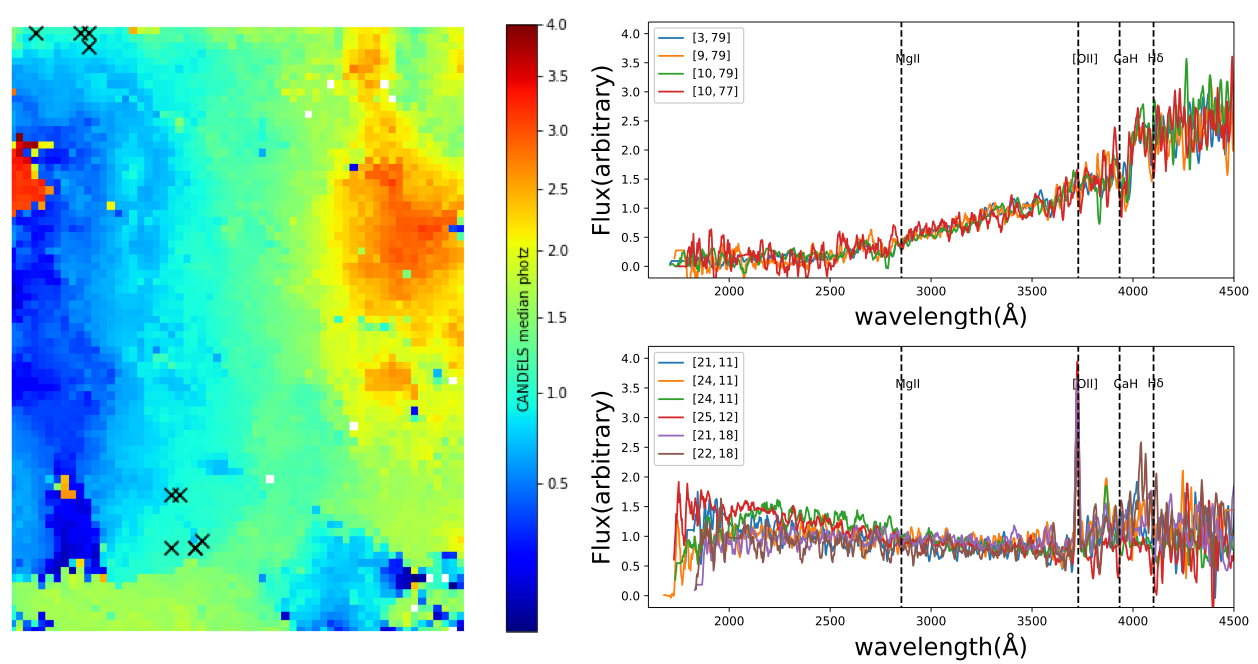
\includegraphics[width=\textwidth]{figs/Hemmati18_Fig8_VVDS_spec.png}
% %
% \caption{\small {\it Left}: A Self-Organizing Map
% \citep[SOM;][]{1990Natur.346...24K} from \citet{hemmati18} encoding the
% relation between colors in an LSST+WFIRST-like color space and redshift,
% $z$.  Position in the SOM is associated with a position in the
% multi-dimensional broad-band color space of galaxies.  Galaxies observed
% in this space are assigned $z$ values based on the median photo-$z$ of
% galaxies from the CANDELS survey \citep[color
% bar;][]{2011ApJS..197...35G}.  Such SOMs can be used to optimally define
% spectroscopic training samples for use with imaging surveys.  {\it
% Right}: Galaxy spectra from VVDS \citep{2005A&A...439..845L}; black
% crosses near the top and bottom of the SOM are plotted in the top and
% bottom panels, respectively.  Note the similarity of the high-resolution
% spectra associated within the SOM, suggesting that a systematic
% spectroscopic exploration of the LSST color space would have
% far-reaching benefits to the science return of the mission beyond the
% photo-$z$ application.}
% %
% \label{fig:SOM}
% %
% \end{figure}

%-----------------------------------------------------------------------
\subsubsection{Enhancing Dark Energy Probes via Precision Cosmic Distances}
\label{sec:cosmology}

The quest to understand the accelerating cosmic expansion has motivated billions of dollars of investment in efforts world-wide ---
culminating in the ``Stage IV'' dark energy missions LSST, Euclid, and WFIRST --- that seek highly precise measures of cosmic structure to constrain the
evolving dark energy equation-of-state. Delineating the growth of cosmic structure requires measurements of galaxy positions and
gravitational shear as a function of distance over vast cosmic volumes.  For the billions of sources that will be
imaged by these surveys, distances must be derived from photometric redshifts (photo-$z$s). Among other challenges, if the photo-$z$s are inaccurate it can introduce significant errors in cosmological
results (e.g., Huterer et al. 2006). Improving galaxy photo-$z$ estimates through deep, targeted
spectroscopic training and calibration samples would propagate through
to substantially improve the cosmology results of \emph{all} of these missions, for all
cosmological probes, not just weak lensing.

The FOBOS Cosmology Program will play a critical role by training photo-$z$s from sources that are too faint for other
instruments (like PFS) but will dominate the number of galaxies and cosmic volume probed by panoramic deep imaging in
the next decade.  Complete spectroscopic training samples to $i_{AB} = 25.3$ will \emph{increase the LSST's dark energy
figure-of-merit by 40\%} \citep{newman15}. FOBOS's strength in this endeavor goes beyond sensitivity.  With no
``redshift desert,'' thanks to its unique ability to measure spectroscopic redshifts above $z > 1.5$ via rest-frame UV
features, the FOBOS Cosmology Program will dramatically reduce the need for expensive,
space-based\footnote{Ground-based near-IR spectroscopy is too contaminated by sky-line emission to provide spec-$z$s at
the required level of completeness \citep{newman15}.} near-IR spectroscopy.

\chal{photozs}
%
\begin{enumerate}[rightmargin=0.2cm,leftmargin=0.2cm]
%
\item[] {\textsf {\large FOBOS Cosmology Program:}}  For a set of 12
  0.1 deg$^2$ FOBOS pointings arranged evenly in right ascension and
  chosen to overlap with the LSST, Euclid, and WFIRST footprints, this
  program will execute ultra-deep integrations of $\sim$15,000 $24 <
  i_{AB} < 25.3$ sources using 1200 single fibers (per pointing) from
  two of FOBOS's three spectrographs. 
  Fiber-IFUs from the 3rd
  spectrograph will be used for simultaneous Galaxy Program
  observations (see below).  The depth is chosen to be well-matched to the depth of the majority of the LSST and WFIRST
  weak lensing shear sample. To maximize the power of the resulting
  photo-$z$ training sample, we will carefully choose the sample such that it 
  efficiently spans the full LSST/WFIRST color-magnitude space, as described in \citet{masters15, masters19}. We will
  dynamically re-allocate fibers to new targets as successful
  redshifts are obtained (i.e., some fibers will deliver multiple
  spec-$z$s).  The longest integration times per field will exceed 100
  hours.  This program would require 34 dark nights per year for 5
  years. The program, the spectra from which would be reduced and made public immediately, would yield huge scientific returns beyond photo-$z$ training and calibration, as it would naturally double as 
  a highly detailed probe of galaxy evolution over cosmic time. 

\end{enumerate}

%-----------------------------------------------------------------------
% \begin{wrapfigure}{r}{0.5\textwidth}\small
% %
% 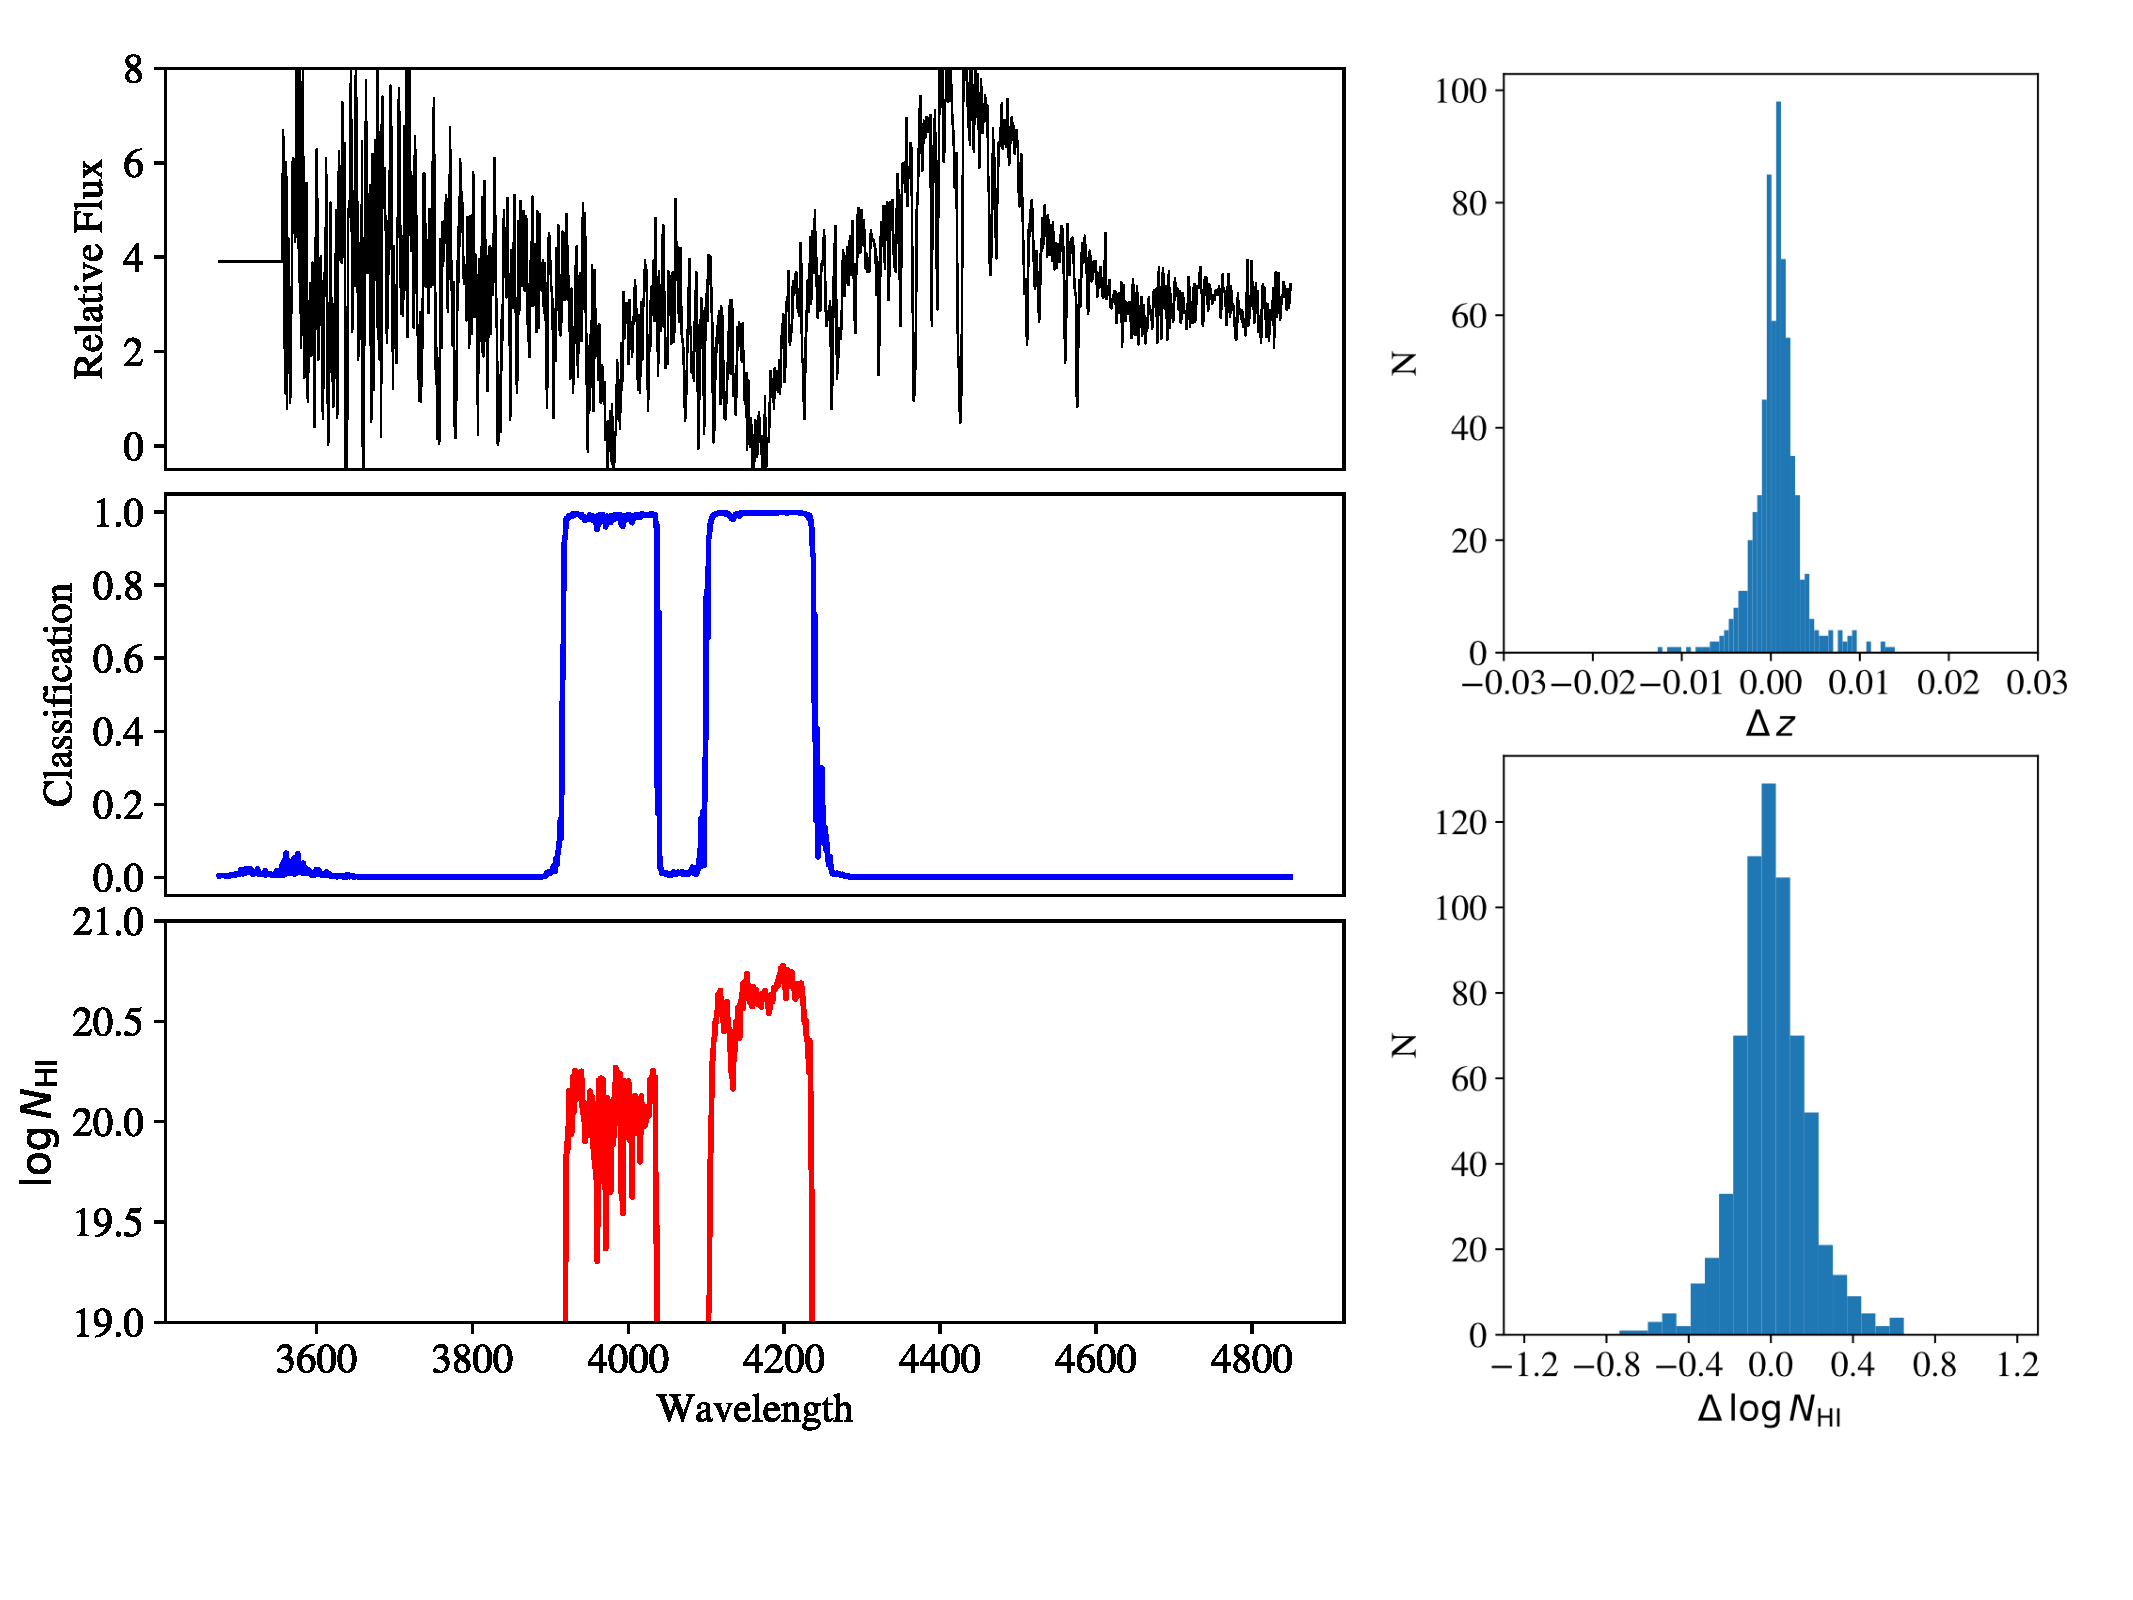
\includegraphics[width=0.5\textwidth]{figs/Parks_fig.pdf}
% %
% \caption{Application of machine learning to find and quantify the
% physical parameters of absorption by neutral hydrogen gas in spectra
% taken along quasar sight lines \citep[adapted from Figs 7 and 14
% from][]{parks18}.  Two absorption systems in the spectrum (top-left) are
% identified (middle-left) and then ``labeled'' with an HI column density
% ($N_{\rm HI}$) (bottom-left) using a convolutional neural network (CNN).
% Redshift, $z$, (top-right) and $N_{\rm HI}$ (bottom-right) measurements
% obtained the CNN are in excellent agreement with derivations by experts.
% FOBOS will provide rich data sets for similar transfer of
% physical parameter labels to photometric and spectroscopic data.}
% %
% \label{fig:absorber}
% %
% \end{wrapfigure}

\subsubsection{Mapping the Baryonic Ecosystem of Early Galaxies at All Scales}
\label{sec:galaxies}

% From George:
% - fill out case for probing both galaxies and their “gas-filled
%   environments”
%    - make it more explicit that getting large numbers of redshifts
%      would make it possible to trace out large-scale structure in
%      detail
%    - enables studies of galaxy properties as a function of environment
%
% - also mention targeting galaxies along QSO lines of sight
%    - much higher target density than with LRIS, DEIMOS over larger FOV.
%
% - Worth discussing Lyman-alpha or metal-line tomography?  
%
% - More quantitative comparisons with existing data sets?
%    - What key science questions can FOBOS address that many years of
%      LRIS and DEIMOS observations have not been able to?  Surely some
%      level of the spectral tagging and photo-z training can be done
%      (and surely is being done) with existing data.  Is FOBOS going to
%      be a huge leap, or will it mainly be cleaning up neglected corners
%      of parameter space?
%
% - More excited to hear about how the FOBOS spectra will be used for
%   science directly, instead of support for LSST

The fueling and regulation of galaxy growth during the peak formation epoch ($z \sim2$--3) is critically tied to the turbulent and gas-rich ecosystem in which early galaxies evolve.  James Webb Space Telescope and Extremely Large Telescopes will marshal powerful infrared observations to study the stars and nebular gas at the heart of these early galaxies.  But to map out their crucial link to the extended gas reservoirs, diffuse halos, and streaming filaments that dominate the mass in these environments requires an instrument like FOBOS.  Its deep sensitivity and high sampling density enables comprehensive tomographic reconstruction of the intergalactic medium (IGM) across the largest cosmic structures in a single pointing ($\sim$10 transverse Mpc at $z \sim 2.5$).  Its blue sensitivity probes Ly-$\alpha$ across the complete formation epoch ($z = 1.5$--3.5) and opens access to high-ionization transitions that reveal diffuse gas \emph{in emission}, such as O VI (1032 \AA).  Finally, its ability to combine single-fiber and multiplexed IFU observations allows us to map the density and dynamical state of diffuse gas at all relevant scales.




systems into the more ordered, star-dominated structures that populate the
universe today.  This period marks the peak of cosmic star formation and galaxy assembly.   To understand it, we must
study the entire galaxy ``ecosystem,'' including not only the galaxies themselves but their gas-filled environments.
The goal is to build a comprehensive picture of the physical processes that fuel proto-galaxy growth, shape their
internal structure, and influence their environment.

Although our first challenge emphasized photo-$z$ training, here we will apply machine learning more broadly to infer
physical parameters from multi-wavelength photometry as well as lower quality spectra trained with high-S/N data sets 
(cf., Fig.~\ref{fig:absorber}).  Given the cost of deep spectroscopy, a central goal is to extract the maximum
information from photometry and shallower spectroscopy so that more statistically powerful samples over larger cosmic
volumes can be studied.

%  build SDSS-like
% statistics for galaxies at this key cosmic epoch.  In all of these
% challenges, we will use simulated data sets to isolate uncertainties and
% biases in various training-set design strategies, including the benefits
% of additional imaging information like morphology and size from a wide
% range of wave-bands (e.g., combining LSST, Euclid, WFIRST).  The
% exercise will define requirements for FOBOS instrument performance and
% the optimal training sample delivered publicly.

% LSST's panoramic imaging will detect huge numbers of galaxies at this
% epoch.  Targeted followup with FOBOS will allow us to ascribe detailed
% galaxy and environmental information from deep spectroscopic training
% samples to the much larger cosmic volumes surveyed with broad-band
% imaging.

\begin{enumerate}[rightmargin=0.2cm,leftmargin=0.2cm]
%
\chal{phot}
%
\item[] {\textsf {\large Data-Science Challenge \ref{phot}: Apply deep-
learning algorithms to infer physical properties of galaxies at
$z$$\sim$2 using using photometry.}} The range of observed spectral
types is well-constrained by broad-band imaging (Figure \ref{fig:SOM}),
suggesting a far greater potential for imaging data to reveal physical
properties with sufficient training than conventional modeling of
spectral energy distributions (SEDs) would suggest.  The challenge here is to identify the extent to which machine
learning can deliver SDSS-like information --- e.g., star-formation histories,
stellar-population properties, dust content, inflow/outflow properties,
and stellar masses --- and determine design parameters for future training sets that will enable such inferences for millions of imaged galaxies at $z$$\sim$2.
%
\end{enumerate}

% \begin{enumerate}[rightmargin=0.2cm,leftmargin=0.2cm]
% %
% \chal{uv}
% %
% \item[] {\textsf {\large Data-Science Challenge \ref{uv}: Infer stellar
% and ISM indicators in UV spectra from rest-frame optical spectra}}.
% There are many powerful gas and stellar spectral features just redward
% of the Lyman-$\alpha$ line at 1216\AA.  By combining FOBOS UV and
% existing near-IR spectroscopy at $z$$\sim$2, we can transfer physical
% ``labels'' determined in the rest-frame optical to spectra at UV
% wavelengths, which will dramatically enhance interpretation of JWST
% discoveries of the first galaxies ($z$$\sim$10) for which rest-frame UV
% imaging and spectroscopy will be most accessible.  A similar application
% can ascribe the escape fraction of Lyman-continuum radiation observed in
% FOBOS spectra to constrain the sources responsible for ``reionization''
% at $z$$\sim$6 \citep[cf.]{2018ApJ...869..123S}.

% % With simulated spectral observations, we will determine the extent of
% % label transfer that is possible and set requirements on training
% % samples.

% \end{enumerate}

\begin{enumerate}[rightmargin=0.2cm,leftmargin=0.2cm]
%
\chal{lowsnr}
%
\item[] {\textsf {\large Data-Science Challenge \ref{lowsnr}: Train
short spectroscopic exposures in combination with photometry to provide
environmental diagnostics for 1M galaxies at $z$=1--2}}.  Photometric
redshifts, while acceptable in large cosmological analyses, wash out
information about the local position of galaxies with respect to one
another.  To characterize a galaxy's local environment and identify its
neighbors requires (observationally expensive) spectroscopic redshifts.  However, with improved photo-$z$s available
from Challenge \ref{photozs} and strong priors on spectral types
(Challenge \ref{phot}), the challenge here is to push machine-learning techniques to deliver
\emph{spectroscopic} redshifts (with 300 km s$^{-1}$ accuracy) at the lowest signal-to-noise possible.  Reductions by
factors of 4--5 in exposure time would enable FOBOS to complete a 1M galaxy environment survey at $z=1$--$2$ in just
20-30 nights.

\end{enumerate}

% \begin{figure}[h!]
% %
% \vskip -0.1in
% %
% 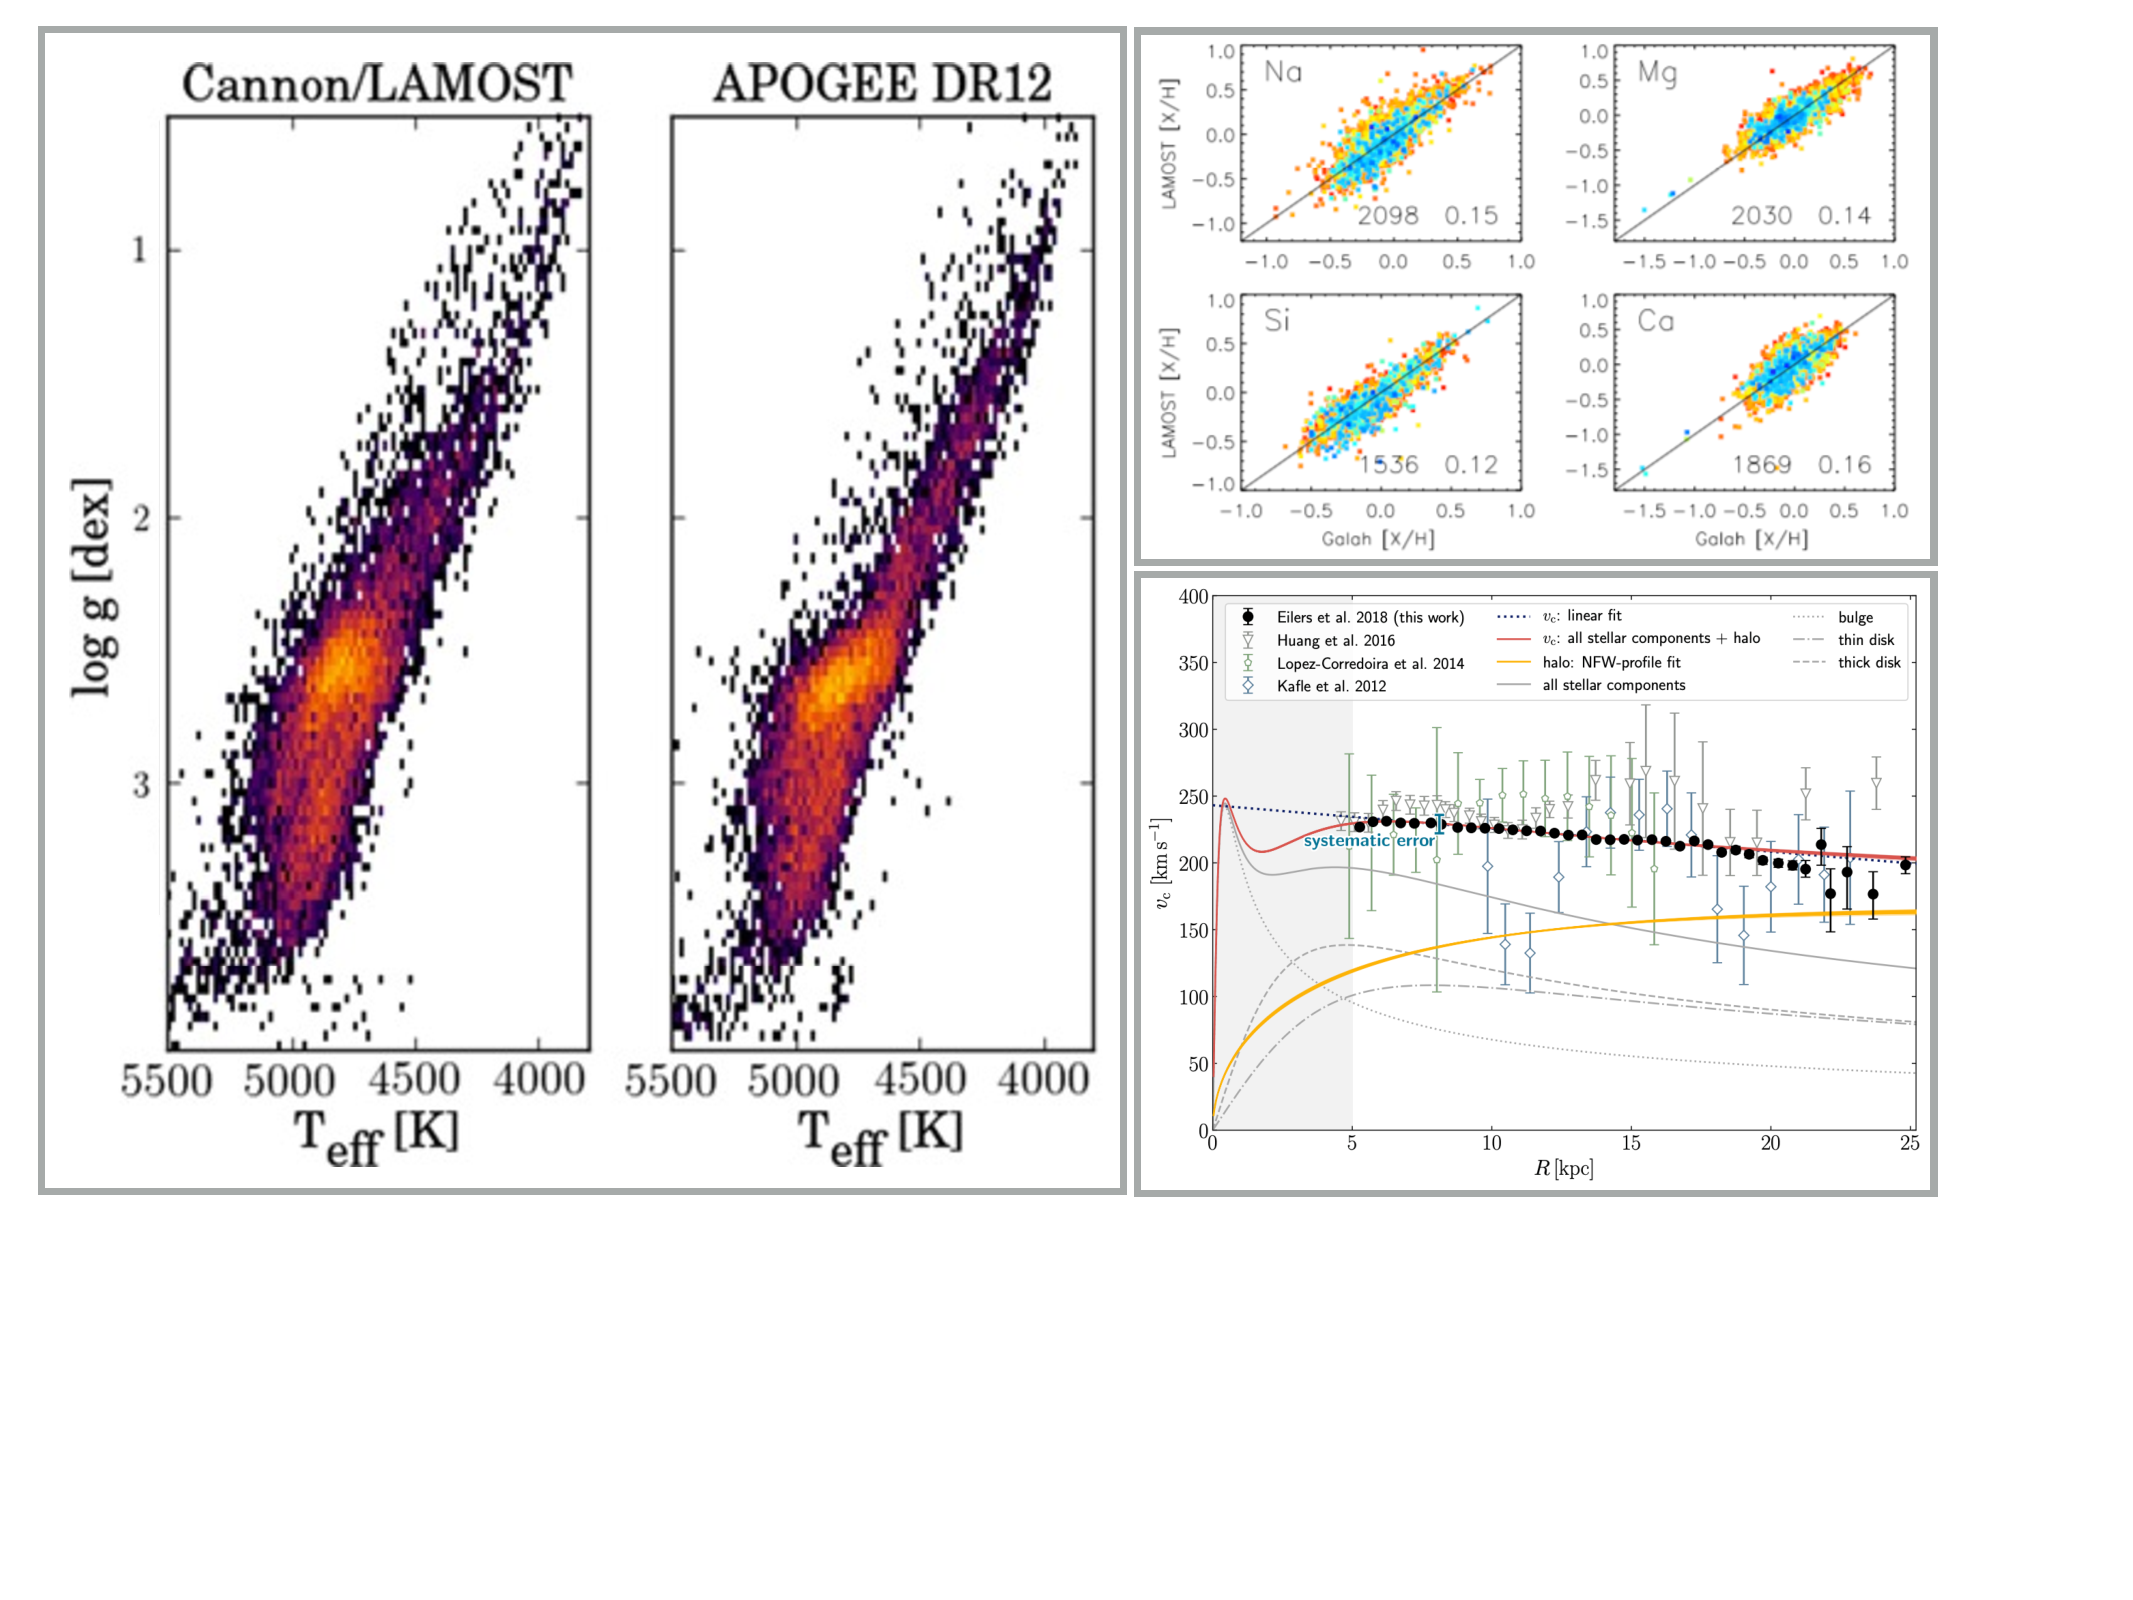
\includegraphics[width=\textwidth]{figs/LGplots}
% %
% \caption{{\it Left}: Validation of {\it The Cannon} measurements of
% stellar effective temperature, $T_{\rm eff}$, and surface gravity, $\log
% g$, using low-resolution LAMOST spectra (left) compared to
% high-resolution APOGEE measurements
% \citep[right;][]{2017ApJ...836....5H}. {\it Top-right}: Recovery of
% elemental abundances from low-resolution LAMOST spectra compared to
% high-resolution measurements from GALAH (Xiang et al., in prep).  {\it
% Bottom-right}: The circular-speed curve of the Milky Way determined
% using a data-driven model that combines stellar parameters determined
% from APOGEE spectra with photometry from WISE, 2MASS, and Gaia, yielding
% the most precise measurements to date \citep{2019ApJ...871..120E}.}
% %
% \label{fig:Cannon}
% %
% \end{figure}

%-----------------------------------------------------------------------
\subsubsection{Unraveling the Formation History of our Local Group of Galaxies}
\label{sec:localgroup}

Our Local Group of galaxies---the Milky Way (MW), the Magellanic Clouds,
Andromeda (M31) and Triangulum (M33) Galaxies, and a multitude of
satellite galaxies---allows us to study one realization of the galaxy
formation process in superb detail.  In the next decade, LSST and WFIRST
will increase the census of stellar streams and halo substructure in
these galaxies by a hundredfold.  Follow-up \emph{stellar} spectroscopy
will constrain stream orbits and the total mass they enclose
\citep{2017ApJ...836..234S} as well as the associated age and chemical
composition (see below).
%\citep{2019MNRAS.484.3425M}.
As theoretical modeling also advances, these new data promise exciting
insights on the formation history of the Local Group.

Radial velocity studies of stars in the MW halo or the M31 disk require
observations of up to 10 hours on large telescopes
\citep[e.g.,][]{2018arXiv180904082C}.  This again motivates
machine-learning algorithms to extract physical quantities from both
multi-band imaging and lower quality spectra (low resolution and S/N)
using relatively small, yet high-S/N, training sets.  For example,
\citet{2015ApJ...808...16N} have developed {\it The Cannon}, a
supervised learning approach that uses spectra with known stellar
parameters to label spectra where those parameters are unknown
(Fig.~\ref{fig:Cannon}).  Additionally, \citet{2018arXiv180401530T} have
developed {\it The Payne} which can infer 16 stellar-abundance labels
from low-resolution spectra using a neural network and theoretical
stellar spectra.  Finally, \citet{2018arXiv180803278T} have combined
Kepler-based astroseismology measurements with APOGEE spectra to
determine stellar age to $\sim$25\% precision using a neural network.
Our proposed effort builds on new lines of inquiry based on these
successes.

\begin{enumerate}[rightmargin=0.2cm,leftmargin=0.2cm]

\chal{stellar} 
%
\item[] {\textsf {\large  Data-Science Challenge \ref{stellar}: A nested network of stellar parameter training
samples for resolved Milky Way and Local Group studies.}}  As in our other challenges, the key driver here is the
ability to extract maximum information from photometry, in this case stellar parameters.  Our goal is to reach
magnitudes significantly fainter than the detection limit of current and upcoming spectroscopic surveys of the Milky
Way including Gaia, APOGEE\footnote{APOGEE, the Apache Point Observatory Galaxy Evolution Experiment has observed in
both SDSS-III and SDSS-IV.}, the SDSS-V Milky Way Mapper, planned programs with 4MOST\footnote{4MOST: 4-meter
Multi-object Spectroscopic Telescope.} and the Dark Energy Spectroscopic Instrument (DESI) Milky Way Survey, among
others. Inferring
stellar parameters beyond V$\sim$18 will open up studies of the Milk Way's outer halo, the halo of M31, and stellar
populations in local dwarf galaxies.

The immediate challenge is to design an optimized, nested set of training samples that connect data from the surveys
above.  This nested set will span high-S/N to low-S/N and high spectral resolution to low spectral resolution for
sufficiently large, overlapping stellar samples.  Subsets will have astroseismology from TESS\footnote{TESS is NASA's
Transiting Exoplanet Survey Satellite.} and PLATO\footnote{PLATO is ESA's PLAnetary Transits and Oscillations
mission.}.  Using simulated spectra with known input parameters, we will test methods for ``label transfer'' from
information-rich spectra to information-poor spectra as we work down to fainter magnitudes, landing eventually at
multi-band photometry alone. Within this nested set, low-resolution FOBOS data will fill in gaps at both high-S/N,
where we will be training FOBOS data on higher resolution spectroscopy, as well as lower-S/N where we will be training
photometry on FOBOS spectroscopy.  The success of this multi-layered label transfer depends not only on the size of the
training sets we can access or observe, but on how representative they are.  Label transfer to WFIRST imaging of the
M31 halo, or Local Group dwarfs in either hemisphere, is a particular concern.  We will test it by evaluating label
recovery on simulated stellar spectra with cosmologically-informed formation histories for M31 and dwarf galaxies,
suitably differentiated from the Milky Way stars that anchor the training network.



% \chal{mwhalo} 
% %
% \item[] {\textsf {\large  Data-Science Challenge \ref{mwhalo}: The
% chemical evolution and assembly history of the MW stellar halo.}}  Using current MW halo models, we will simulate FOBOS
% stellar spectroscopy of main-sequence turn-off
% and red-giant stars in these substructures within the MW that also
% leverages existing data from, e.g., APOGEE and H3.  We will build
% data-driven models based on these data to measure stellar parameters
% (temperature, surface gravity, metallicity, and alpha-element abundance)
% for all halo stars with LSST+2MASS+WISE+WFIRST multi-band photometry,
% allowing us to reconstruct the star-formation history of each disrupted
% satellite. These will be combined with dynamical data and compared with
% cosmological simulations to build a generative model for the assembly
% history of the MW stellar halo.

% \chal{m31} 
% %
% \item[] {\textsf {\large Data-Science Challenge \ref{m31}: The
% differential chemical evolution of M31 and MW.}}  A natural extension of
% Data-Science Challenge \ref{mwhalo} is to perform the same analysis for the
% halo of M31.  However, we cannot expect to obtain high-quality spectra
% of individual main-sequence stars at the distance of M31 with FOBOS.
% Moreover, training a chemical evolution model using spectra of Milky Way
% stars may lead to systematic errors:  The Milky Way and Andromeda have
% distinct evolutionary histories \citep[e.g.][]{2005MNRAS.356.1071R},
% despite being relatively similar in many other respects.  We will
% therefore obtain deep observations of giant stars in the M31 halo to
% drive a machine-learning algorithm that combines a model of the MW halo
% with results from cosmological hydrodynamical simulations to constrain
% the differential history of the MW and M31 stellar halos.

% \chal{gaia} 
% %
% \item[] {\textsf {\large Data-Science Challenge \ref{gaia}: Stellar
% parameter determinations for a billion stellar spectra.}} While
% providing on-sky motions and photometry for 1.7 billion stars in the MW,
% fewer than 10\%, 0.3\%, and 0.1\% of stars will have a full complement
% of astrometrics and kinematics, basic stellar parameters, and chemical
% abundances, respectively.  Moreover, Gaia distance errors increase
% quadratically with distance.  To realize Gaia's full potential, we will
% design FOBOS training sets that, when combined with high-resolution
% datasets from, e.g., APOGEE, WEAVE, will allow us to build data-driven
% models of the absolute magnitude (yielding distance modulus),
% temperature, surface-gravity, and stellar abundance for {\it all} stars
% in the Gaia dataset.  These data will allow us to isolate coeval
% populations in the Galactic disk that can be combined with very
% high-resolution simulations of the Milky Way to provide a detailed
% evolutionary history of our Galactic home.

\end{enumerate}

%-----------------------------------------------------------------------
%-----------------------------------------------------------------------
\section{Project Implementation}
\label{sec:project}

To meet the substantial spectroscopic needs of the U.S.\ astronomy
community (Section \ref{sec:community}), we propose three coordinated
activities: 1) Organizing and evaluating the results of a community-wide
effort to address a series of data-science challenges; 2) Completing
preliminary design for the FOBOS instrumentation, informed in part by
refining requirements as a result of (1); 3) Designing the operational
modes, planning tools, data analysis software, and platforms necessary
to deliver public training data that address these challenges.  We focus
our current request on the Preliminary Design Phase (PDP) of FOBOS
development, following the the overall project plan and final
deliverables outlined below.  Anticipating progress in all three
activities, we will request NSF MSRI-2 funding in 2021 to build and
deploy FOBOS at WMKO, with observations and publicly served training
data to follow.  FOBOS would see first light in 2027 and carry a total
cost of \$32M (without contingency in 2019 dollars).

\subsection{FOBOS Instrument Concept}
\label{sec:concept}
% \noindent \comment{1 page}

% Here's an alternative way to put in figures if we want captions on the side (to save space)
% Could introduce a new ``counter'' to count and label figures appropriately
%\centerline{\hbox{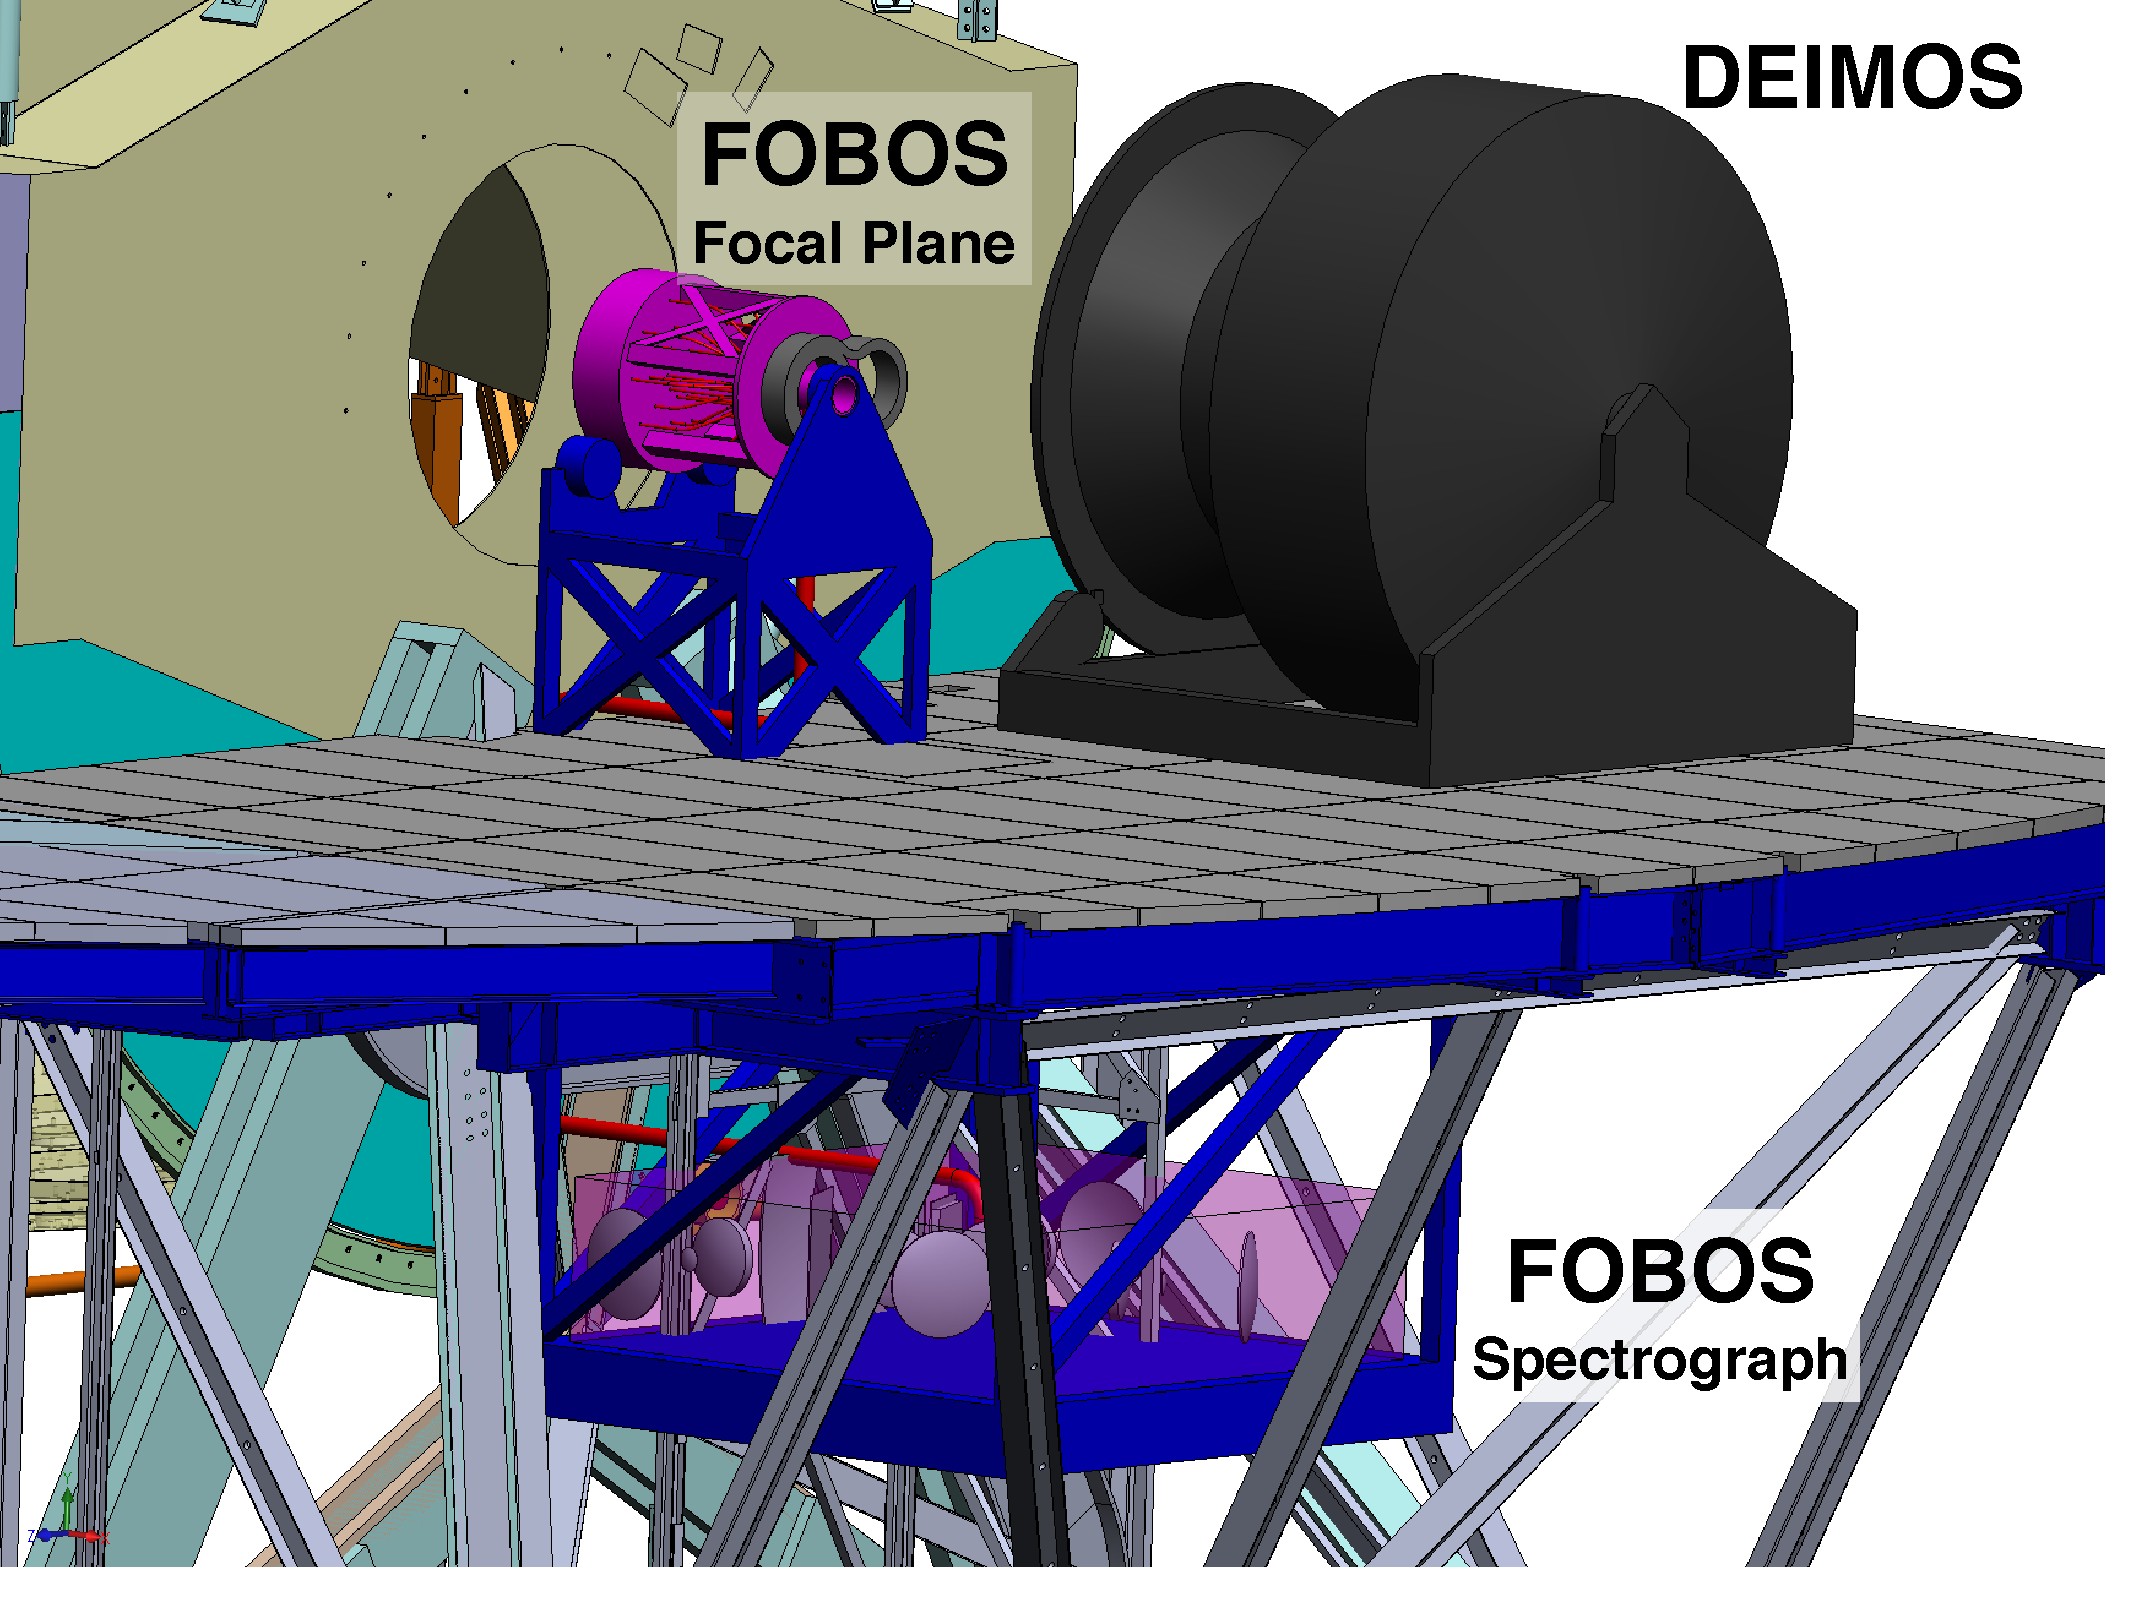
\includegraphics[width=0.6\textwidth, angle=0]{figs/FOBOSatKeck_v1.pdf}
%    \hspace{0.1cm} \vspace{2in}
%    \parbox[b]{0.3\textwidth}{\small {\bf Figure ??:} Rendering of FOBOS instrument systems deployed at the Keck II Nasmyth port.  By mounting the FOBOS spectrographs under the Nasmyth platform, other instruments like DEIMOS can maintain access to the telescope. \vspace{2cm}}}}

\begin{figure}[h!]
%
\vskip -0.1in
%
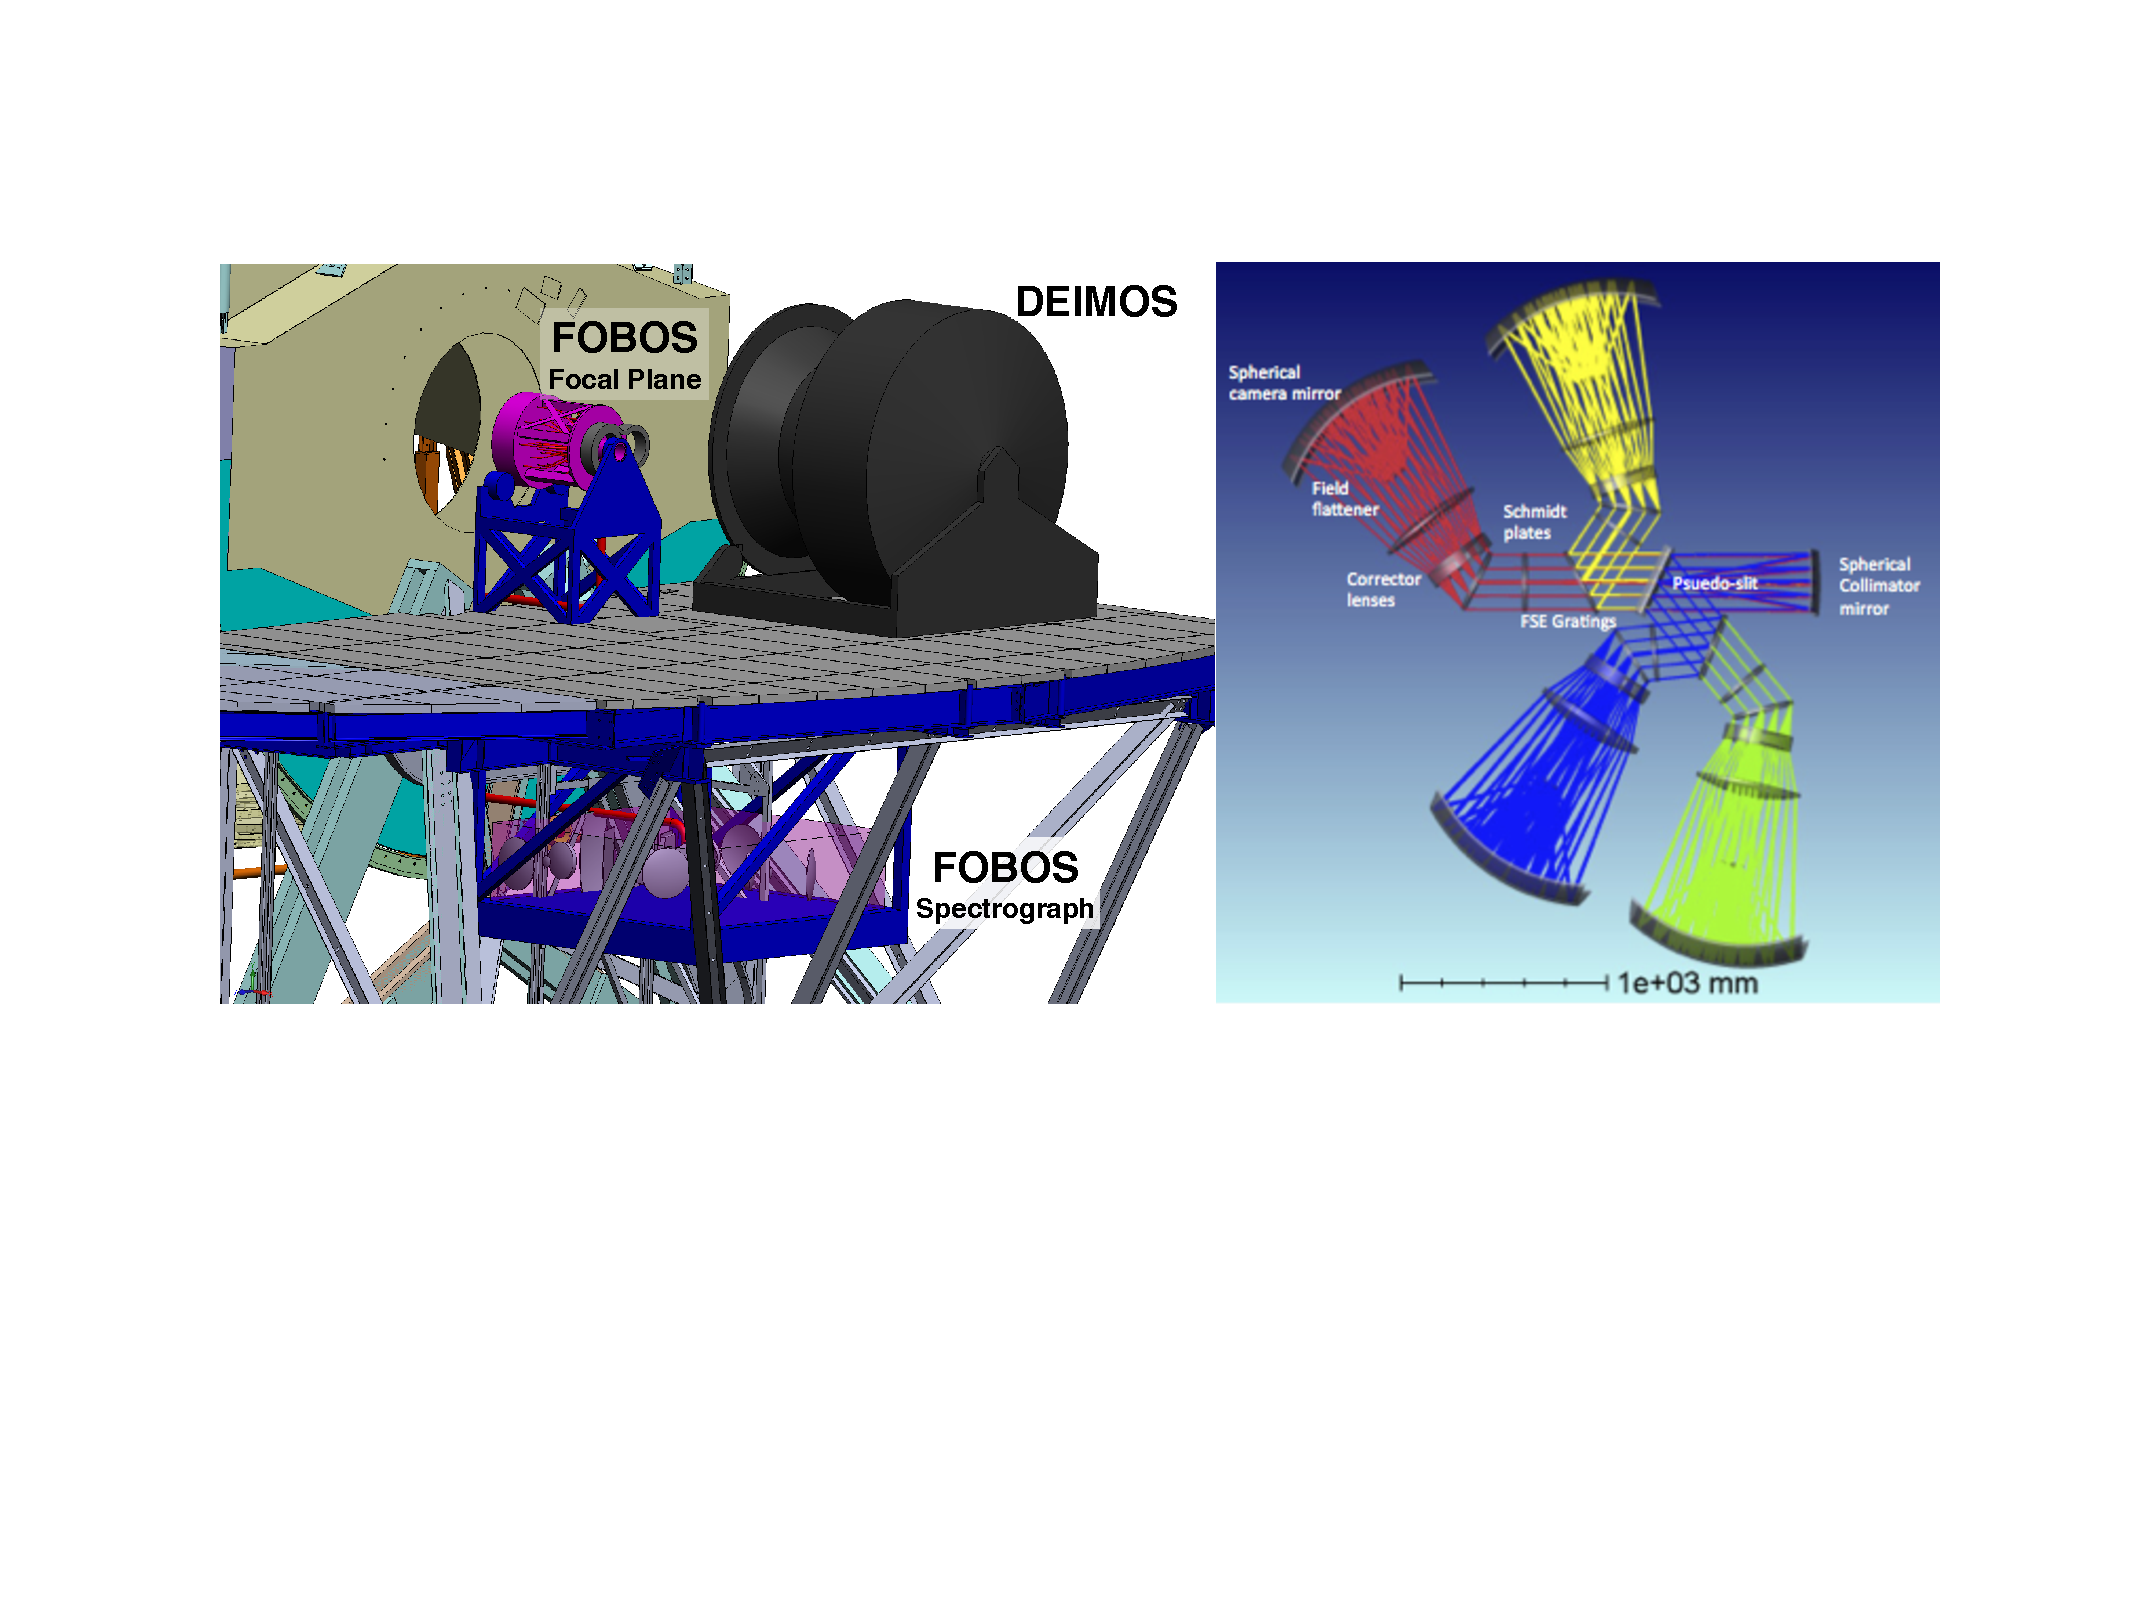
\includegraphics[width=\textwidth]{figs/FOBOS_inst.pdf}
%
\caption{\small {\it Left}: Rendering of FOBOS instrument systems
deployed at the Keck II Nasmyth port.  By mounting the FOBOS
spectrographs under the Nasmyth platform, other instruments like DEIMOS
can maintain access to the telescope. {\it Right}: Rendering of one of
the three four-armed FOBOS spectrographs.}
%
\label{fig:layout}
%
\end{figure}

Mounted at the Nasmyth focus of Keck II Telescope at WMKO, FOBOS (Fig
\ref{fig:layout}) will be one of the most powerful spectroscopic
facilities deployed in the next decade.  FOBOS includes a compensating lateral
atmospheric dispersion corrector (CLADC, not pictured) to ensure that
target light from all wavelengths falls on allocated fibers while also
correcting image aberrations at the edges of the 20 arcmin diameter Keck
field.  Each of the CLADC lenses is 946 mm in diameter, the first two
closely spaced with lateral relative motions enabled by three
barrel-mounted actuators.  The final CLADC lens surface serves as the
vertical mounting plate for roaming Starbugs fiber positioners.  It
translates to track focal plane tilt.  Starbugs patrol a large on-sky
area ($\sim$1 arcmin), enabling flexible and dynamic targeting
configurations with adjacent fibers as close as 10 arcsec.

A total of 1800 150-$\mu$m core diameter fibers are deployed at the curved focal plane.  Fore-optics on the front end
of each fiber demagnify and speed up the beam (from f/15 to f/5) for better coupling to the fiber numerical aperture
and to minimize losses from focal ratio degradation.  The focal plane plate rotates and translates to follow image
positions as the telescope tracks across the sky.  The fiber run is kept at less than 10m to maintain high throughput
at UV wavelengths.  Special care is given to stress-relief cabling to minimize variable focal ratio degradation over
the fiber run.

Sets of 600 fibers feed each of three identical spectrographs (Fig
\ref{fig:layout}).  Each spectrograph uses a series of dichroics to
divide the 259 mm diameter collimated beam into four wavelength channels with combined, instantaneous
coverage from 0.31--1 $\mu$m.  Fused-silica etched (FSE) gratings provide mid-channel spectral resolutions of $R
\sim 3500$ at high diffraction efficiency in each channel.  The dispersed light is focused by an f/1.1
catadioptric camera\footnote{Based on the camera design for the Multi-Object Optical and Near-infrared Spectrograph (MOONS) on the Very Large Telescope (VLT).} and recorded by an on-axis 4k$\times$4k CCD mounted
at the center of the first camera lens element.  Spectrographs are
mounted in a temperature controlled housing installed under the Nasmyth
Deck to allow space for other Keck instruments above.  The end-to-end
instrument throughput peaks at 60\% and is greater than 30\% at all wavelengths
%\comment{compare to PEP}.

FOBOS includes observatory level systems for precise instrument
calibration using dome-interior screen illumination, a metrology system
for accurate fiber positioning, and guide cameras for field acquisition
and guiding.  The instrument design envisions future upgrades including
alternate collecting modes that deploy multiple fiber bundles, feeds to
other fiber-based spectrographs at different wavelengths or spectral
resolutions, and the ability to support and benefit from image
corrections with Ground-Layer Adaptive Optics.

\subsection{FOBOS Instrument Design Effort}
\label{sec:design}

FOBOS will complete its current conceptual design phase in fall 2019. Funding from this proposal will support the next
phase of Preliminary Design.  A schedule of milestones and additional information is provided in the Project
Execution Plan (PEP).  Major components of the Preliminary Design effort are described below.

\noindent \textbf{Atmospheric Dispersion Compensator (ADC):} The
opto-mechanical design, tolerancing, lens cell design, motion systems,
and software-control design of the ADC will be completed.  

\noindent \textbf{Focal Plane System:} Mechanical design, including flexure analysis and
the selection of drive mechanisms and potential vendors will be
completed.  This system also defines one of the interfaces to the Keck
II Telescope and must comply with WMKO space envelopes, servicing needs,
and other requirements.  The focal plane system also includes the
guide cameras.

\noindent \textbf{Starbugs fiber positioners:} Starbugs are a
positioning technology developed and deployed by the Australian
Astronomical Observatory (AAO), which has partnered with our team to
generate a conceptual design for use of Starbugs by FOBOS.  Design
requirements for Starbugs in FOBOS are more relaxed than the currently
on-sky TAIPAN instrument thanks to the larger physical plate scale at
Keck.  

\noindent \textbf{Fiber System:} We will complete the optical design and
processing plan for affixing forward optics lenses to each fiber head.  A
micro-lens array solution will be developed for a central,
fixed-position 4.5-arcsec diameter IFU for fast source acquisition. This
work package also includes the stress-relief cable system and fiber
termination hardware and processing.

\noindent \textbf{Spectrographs.} The optical systems and components
(slit, collimator, dichroics, gratings, and camera), an analysis of
acceptable tolerances and performance, their mechanical supports,
software controls, and the overall enclosure will all be advanced
through Preliminary Design.  Detectors, cryostats, read-out electronics
and systems for thermal management will be designed.

% Put the calibration system back in?
% \noindent \textbf{Calibration System.} This package includes design of an interior dome screen and projection system for injecting calibration sources with sufficient spatial uniformity and stability into the instrument.  We will work with the Observatory to develop an integration and controls plan.  No such calibration system currently exists at Keck.

% \noindent \textbf{Auxiliary Systems.} Design of auxiliary systems includes Nasmyth platform interfaces, utilities access, fiber routing and support, thermal control and vibration control systems.

\subsection{Addressing Data Science Challenges and Designing FOBOS Training Sets}
\label{sec:survey}

Our team includes leading experts on data science applications to
astronomy and, specifically, LSST.  We will also use our established
connections to LSST's Informatics and Statistics Science Collaboration
(ISSC) to advertise, recruit, and coordinate efforts to tackle the Data
Science Challenges described in Section \ref{sec:goals}.  Our proposal
request includes two community workshops to motivate progress and discuss
results. At the end of the proposal period, we will publish the results
and developed software packages.

Our data-science challenges require work on simulated
imaging$+$spectroscopic data sets where input physical properties (e.g.,
redshift) can be compared to output recovered values.  Simulated imaging
data (e.g., from LSST and WFIRST) are in-hand, while mock spectroscopy
will be provided by a FOBOS instrument simulator, an initial version of
which has already been developed.  Further advances to be supported by
this proposal include improved error modeling and simulating systematic
effects from detector artifacts, image quality aberrations informed by
the emerging detailed optical design, and variable observing conditions.

The resulting success in addressing each data-science challenge will
define a level of readiness and set requirements on desired FOBOS
training sets, including number of sources, pointings, magnitude limits,
signal-to-noise thresholds, and observing conditions.  Preliminary
observing design and a description of required operational modes to
efficiently observe these training sets will begin with this proposal.
Operational modes will set requirements on target aggregation and
prioritization systems, field acquisition speed, field rotation range,
zenith avoidance zone, reconfiguration time, calibrations, read-out
time, quick-look reduction software and processing rates.  We will
develop integrated program concepts that efficiently combine required
observations.  Detailed survey and execution plans will be completed in
the next phase of this project (MSRI-2).  Roughly 20\% of Keck observing
time is open to the public, and as in previous federally-funded
projects, we fully expect that Senior Personnel at Keck institutions
will be successful in collaborative efforts to secure significant
amounts of additional telescope observing time to enable rapid, public
release of FOBOS training data \citep[e.g.,][]{newman13}.

% The complete photo-$z$ training survey described in \citet{newman15}
% would require 15 independent pointings, each spanning 0.1 deg$^2$ with
% a target density of 6 arcmin$^{-2}$ (8 arcmin$^{-2}$ when including $z
% > 1.5$ galaxies accessible in the UV with Keck-FOBOS), perfectly
% matched to the Keck-FOBOS field-of-view and target density.  With a
% conservative exposure time of 100 hours to reach 75\% redshift
% completeness for 40,000 galaxies with $i_{\rm AB} < 25.3$, the Neman
% survey would require 400 nights.  Challenge \ref{photoz} would reduce
% the required survey duration by a factor of at least four.  Meanwhile
% the extreme depths and flux-limited selection are likely also
% requirements for training sets associated with Challenges \ref{phot},
% \ref{uv}.

% A wider and shallower survey component is envisioned for Challenges
% \ref{lowsnr} and \ref{gaia}.  With 10-minute integrations, a 52
% deg$^2$ Keck-FOBOS sample of environmental diagnostics for 1 million
% galaxies could be carried out in less than 20 nights.  This program
% would sample at $z \sim 1.5$ the same cosmic volume as SDSS.  A
% program of a similar scale would provide training set data for
% inference of stellar parameters in the Milky Way.  These shallow
% programs would be integrated with the deeper components described
% above into a single survey plan.

\subsection{MAISTRO: Target Allocation with Artificial Intelligence}
\label{sec:targeting}

Powered by Starbugs fiber positioners, FOBOS will enable fast, dynamic
reallocation of fibers.  To efficiently determine the best options given
a wide range of possible targets and desired observing outcomes, we will
develop a preliminary design for MAISTRO\footnote{MAISTRO: Modular
Artificial Intelligence System for Target Reallocation and Observing.}
an ``artificial intelligence'' (AI) targeting system that will learn
optimization strategies for assigning targets from a database of
overlapping observing programs with pre-defined priorities.  The AI
package will aggregate data quality using a quick-look reduction
package, science-driven performance metrics, {\it and real-time
assessments of the observing conditions} to make dynamic targeting
recommendations.  For example, if conditions are slightly less than
optimal, MAISTRO would reconfigure Starbugs to brighter objects in a
field or implement a different program prioritization.  MAISTRO will
incorporate updated target lists and priorities from the active observer
and could easily be over-ridden at any time.   Fractions of the full
FOBOS multiplex might also be reserved ``manual targeting'' as required
by the program PI.  

%   - maintains a database with observational progress on individual
%     targets in the survey and
%   - dynamically reallocates fibers based on real-time assessments of
%     the aggregate S/N of each target to meet the specific need of each
%     science case.

% This requires significant design and testing of a combined software
% package and hardware interface.  Specific considerations involve (1)
% fast and robust reduction procedures (cf. MaNGA DOS) that can assess
% the aggregate data and (2) a responsive database with a schema
% optimized for real-time decision making to select targets for
% (re)acquisition while accounting for collision limitations.  Provided
% enough design effort, this lends itself to a machine-learning
% application.

\subsection{Publicly Available Automated Data Products}
\label{sec:DAP}

While the FOBOS data simulator is required for our data-science challenges, it also forms the basis of a delivered data
reduction pipeline (DRP) for this instrument.  This software will provide both the quick reduction assessments needed
for dynamic targeting, as well as full reductions for scientific analysis.  In the proposal period, we will also develop a preliminary design for a data analysis
pipeline (DAP).  Unique among Keck instruments, the FOBOS DAP will take advantage of the fixed spectral format and common target classes to provide high-level data products, including
Doppler shift, emission-line strengths, and template continuum fits (cf.,
Westfall et al.; SDSS-IV MaNGA DAP).  The DAP will also produce results from relevant machine-learning applications (e.g., redshifts at low-S/N).

Raw data, reduced spectra, and high-level DAP science products will be
publicly delivered via user-friendly platforms built on the Keck Observatory Archive.  After associated
proprietary periods, data will be served for {\it all} FOBOS observations, creating a rich legacy data set for the astronomical community.  Both program PIs
and the larger community will be encouraged to develop the DRP and DAP
to meet the needs of specific science applications.  These software
packages will be open source and publicly served (e.g., using GitHub).

\section{Broader Impacts}
\label{sec:bi}

\subsection{Akamai: Training the next generation of Hawaiian STEM
professionals} Led by the Institute for Scientist and Engineer Educators
(ISEE) at UCSC, the Akamai Internship Program is aimed at advancing
college students from Hawai'i into the STEM workforce.  Almost 400
students have participated to date, of which 24\% are Native Hawaiian
and 38\% are women. A longitudinal study of Akamai outcomes indicated
that 87\% were still in STEM, either in the workforce or continuing STEM
studies \citep{asee_peer_31030}.  ISEE and the Akamai program already have deep connections to WMKO; 45 interns have
worked on projects related to instrument
development and observatory operations over the past 15 years.  Our
funding request includes support for two Akamai interns.\footnote{
%
At UCO, an Akamai intern during Summer 2018 helped build a fiber
test-bench at UCSC.}
%
One intern will develop aspects of the FOBOS instrument simulator and use this simulator to develop performance metrics
for the Preliminary Design.  The second will build machine-learning tools for Data-Science Challenge \ref{lowsnr},
specifically for obtaining spectroscopic redshifts at low S/N.


\subsection{Investing in future educators} Also via the ISEE, we will
support three graduate students to participate in the Professional
Development Program (PDP) that build teaching skills through
collaborative design of an inquiry activity.  The PDP team conceives,
develops, and tests the activity which culminates in a lab exercise
run with undergraduates. The program
emphasizes inclusive and equitable learning environments.  Specifically, our team of graduate
students will develop a lab unit related to FOBOS instrument development aimed at
incoming community college transfer students enrolled in UCSC's
highly-successful Lamat Program.  In addition to enriching graduate
student training, these efforts will positively impact 25
undergraduates from California community colleges, a large fraction
from underrepresented minority groups.

\subsection{Student Training} UCSC's {\bf Astro 9} course introduces scientific research methods to 1st-year students
by engaging small student teams on actual research projects supervised by graduate students,
postdocs, and staff.  The {\bf Science Internship Program} (SIP) creates a similar environment for high-school students
 over a 10 week summer program.  We will design projects for both programs focused on simulating data sets and
 introducing machine learning concepts used in our Data Science Challenges.  Both PI Bundy and co-PI Westfall have
 served as research mentors in these programs.

\newpage

\setcounter{page}{1}
\bibliographystyle{nsf}
\bibliography{../../references}

\end{document}


